% !TeX root = HistoricalDesign.tex
% Historical record only; not a current submission.
\documentclass[11pt,a4paper]{article}

\usepackage[T1]{fontenc}
\usepackage[utf8]{inputenc}
\usepackage{lmodern}
\usepackage{microtype}
\usepackage[a4paper,margin=2.5cm]{geometry}
\usepackage{setspace}
\usepackage{booktabs}
\usepackage{longtable}
\usepackage{tabularx}
\usepackage{xcolor}
\usepackage{tikz}
\usetikzlibrary{arrows.meta,positioning,shapes.geometric}
\usepackage[section]{placeins}
\usepackage{natbib}
\usepackage[hidelinks]{hyperref}
\usepackage{float}
\usepackage{array}
\usepackage{graphicx}
\usepackage{enumitem}  %
\usepackage[most]{tcolorbox}

\setstretch{1.08}
\setlength{\parindent}{0pt}
\setlength{\parskip}{0.55em}
\renewcommand{\arraystretch}{1.15}
\newcommand{\placeholder}[1]{\textcolor{gray}{[TODO: #1]}}


% BEGIN embedded wordcount.tex
\newcommand{\mainwordcount}{2017}

% END embedded wordcount.tex



\begin{document}
\begin{center}
{\Large\bfseries Group Q -- Earlier Self-Assessment Design Notes\par}
\medskip
{\large Historical design record\par}
\end{center}
\noindent This document retains the earlier Assess, Check \& Learn and Query design. The project direction described by the user on 12 October 2026 focuses on research similarity and distinctiveness; these earlier modules are not the current agreed scope. Four-member confirmation of the revised design is recorded separately in the project alignment board.

% BEGIN embedded Mock-up.tex
% PHASE 2 DESIGN ADDENDUM. Team members may edit their named blocks below.
% This is a proposed mock-up, not a deployed or validated TU/e service.
\clearpage
\section{Phase 2 Mock-up: Screen Walkthrough and Design Rationale}
\label{sec:phase2-mockup}

\subsection{Home screen: choose a module}
\label{sec:phase2-home}
The prototype opens with three menu choices. The walkthrough below sketches each route; the Check \& Learn screen is a proposed interpretation of its module description for the responsible teammate to review. All records and figures shown in the walkthrough are fictional demonstration data, not measured TU/e results.

\begin{tcolorbox}[colback=gray!3,colframe=black!55,title={Home --- AI for a Greener Research Future},breakable]
\textbf{What would you like to do?}\par\medskip
\fbox{\textsf{1. I want to Assess}}\quad
\fbox{\textsf{2. I want to Check \& Learn}}\quad
\fbox{\textsf{3. I want to Query}}\par\medskip
\textbf{Selected route:} Option 1 opens Section~\ref{sec:assess-dialogue}; Option 2 opens Section~\ref{sec:learn-dialogue}; Option 3 opens Section~\ref{sec:query-dialogue}. A researcher can return here from any route.
\end{tcolorbox}


% BEGIN embedded Assess interaction module.tex
% Included by Mock-up.tex. Every project record and number below is fictional demonstration data.
\subsection{Option 1 --- I want to Assess: a guided project assessment}
\label{sec:assess-dialogue}
This walkthrough uses a laboratory battery-sample project to show where fixed controls, AI assistance and a short conversation each help. The same sequence could ask different activity-specific questions for GPU computation or a printed prototype. The tool proposes an activity type and follow-up prompts; the researcher confirms them. Arithmetic uses recorded quantities, not an AI-generated score.

\newtcolorbox{assessscreen}{enhanced,breakable,colback=green!4,colframe=green!45!black,
  boxrule=0.6pt,arc=2mm,left=3mm,right=3mm,top=2mm,bottom=2mm,
  before=\par\noindent,after=\par\medskip}
\newtcolorbox{assessuser}{enhanced,colback=blue!5,colframe=blue!55!black,
  boxrule=0.6pt,arc=2mm,left=3mm,right=3mm,top=2mm,bottom=2mm,
  width=0.83\linewidth,halign=left}

\subsubsection*{A. Start from the menu and confirm the activity}
\begin{assessscreen}
\textbf{Home $>$ 1. I want to Assess $>$ New assessment}\par
\textbf{Choose a starting point:}\quad
\fbox{\textsf{Battery or laboratory samples}}\quad
\fbox{\textsf{GPU computation}}\quad
\fbox{\textsf{3D-printed prototype}}\quad
\fbox{\textsf{Describe another activity}}\par\medskip
\textbf{Researcher selects:} \fbox{\textsf{Describe another activity}}.
\end{assessscreen}

\begin{flushright}\begin{assessuser}
\textbf{Researcher}\par
I make lithium-ion battery electrode samples. I want to reduce wasted material and electricity without changing which samples count as scientifically valid.
\end{assessuser}\end{flushright}

\begin{assessscreen}
\textbf{AI-assisted draft:} This appears to be a laboratory battery-sample activity. I would assess one batch and one valid sample, while retaining total batch use. Please confirm the activity and define a valid sample.\par\medskip
\fbox{\textsf{Confirm battery-sample activity}}\quad
\fbox{\textsf{Edit description}}\quad
\fbox{\textsf{Choose another activity}}
\end{assessscreen}

\subsubsection*{B. Fill known fields; ask only for a missing condition}
\begin{assessscreen}
\textbf{Project information form --- illustrative prior batch}\par
\begin{tabularx}{\linewidth}{@{}>{\raggedright\arraybackslash}p{0.37\linewidth}X@{}}
Scientific outcome & Electrode samples meeting the same test requirement. \\
Prior batch & 6 attempts; 5 valid samples. \\
Relevant inputs & 60 kWh for the defined batch; 1.2 kg starting material. \\
Boundary and source & Fabrication steps only; fictional lab meter and material log. Upstream production excluded. \\
Personal goal & At most 10 kWh per valid sample, with unchanged quality and safety. \\
\end{tabularx}
\medskip\fbox{\textsf{Confirm fields}}\quad
\fbox{\textsf{Edit amounts or boundary}}\quad
\fbox{\textsf{Mark unknown}}
\end{assessscreen}

\begin{assessscreen}
\textbf{One follow-up question:} What makes a sample valid for this research? The proposed alternative can be compared only if it meets the same requirement.
\end{assessscreen}
\begin{flushright}\begin{assessuser}
\textbf{Researcher}\par
A valid sample passes our existing electrochemical test and safety checks. Keep those requirements for the pilot batch.
\end{assessuser}\end{flushright}

\subsubsection*{C. Review the initial profile and choose an action}
\begin{assessscreen}
\textbf{Initial profile --- before the pilot}\par
The recorded batch used 60 kWh for 5 valid samples, or \textbf{12 kWh per valid sample}. The personal goal is \textbf{10 kWh per valid sample}; the initial gap is \textbf{2 kWh per valid sample above that goal}. Material loss and repeated attempts may be avoidable, but no improvement has yet been observed. Upstream material impacts remain unknown.\par\medskip
\textbf{Suggested action:} Pilot a process change that reduces failed samples; record electricity, starting material, valid samples and test results for the whole batch.\par\medskip
\fbox{\textsf{Plan pilot}}\quad
\fbox{\textsf{Why this advice?}}\quad
\fbox{\textsf{Correct input}}\quad
\fbox{\textsf{Save privately}}
\end{assessscreen}

\begin{table}[H]
\centering\small
\begin{tabularx}{\textwidth}{@{}>{\raggedright\arraybackslash}p{0.20\textwidth}>{\raggedright\arraybackslash}p{0.34\textwidth}X@{}}
\toprule
Criterion & Current evidence & Next check \\
\midrule
C1 Boundary and inputs & Batch, validity rule, meter and material log recorded; upstream excluded. & Confirm the same steps and units in the pilot. \\
C2 Comparable alternative & Process change proposed; quality condition stated. & Test sample performance before claiming a fair comparison. \\
C3 Avoidable use & One failed attempt in the prior batch. & Check whether the change reduces failures or waste. \\
C4 Total use & Batch electricity and material recorded. & Show batch totals alongside per-valid-sample values. \\
C5 Follow-up & Personal goal recorded; result pending. & Set a review date and enter the pilot record. \\
\bottomrule
\end{tabularx}
\caption{Illustrative assessment matrix using the five provisional criteria. These are evidence and action notes, not points to add into a score.}
\label{tab:assess-criteria-screen}
\end{table}

\subsubsection*{D. Optional return: compare the project's own history}
The researcher later selects \fbox{\textsf{My History $>$ Add follow-up}} and enters a fictional pilot batch: 6 attempts, 6 valid samples, 54 kWh and 1.1 kg starting material. The tool first checks that the scientific test, safety requirements and measurement boundary are unchanged. If they changed, it asks for a revised baseline instead of presenting the difference as an improvement.

\begin{table}[H]
\centering\small
\begin{tabularx}{\textwidth}{@{}>{\raggedright\arraybackslash}p{0.29\textwidth}>{\raggedright\arraybackslash}p{0.21\textwidth}>{\raggedright\arraybackslash}p{0.21\textwidth}X@{}}
\toprule
Measure (same batch boundary) & Prior batch & Pilot batch & Change or goal gap \\
\midrule
Valid samples / attempts & 5 / 6 & 6 / 6 & One more valid sample. \\
Batch electricity & 60 kWh & 54 kWh & $-6$ kWh for the batch. \\
Electricity / valid sample & 12 kWh & 9 kWh & $-3$ kWh from own baseline; $-1$ kWh against the 10 kWh goal. \\
Starting material & 1.2 kg & 1.1 kg & $-0.1$ kg for the batch. \\
\bottomrule
\end{tabularx}
\caption{Fictional follow-up display. Differences are pilot minus the stated reference; negative electricity values indicate less use under the same boundary. A goal is a declaration, while the pilot values require recorded evidence.}
\label{tab:assess-history-screen}
\end{table}

\pagebreak
\begin{assessscreen}
\textbf{Your project, so far:} The pilot is 1 kWh per valid sample below your personal goal and 3 kWh below your own prior batch. Total batch electricity is 6 kWh lower. This is a project-specific observed change only if the meter record and quality checks are confirmed. It does not cover upstream impacts.\par\medskip
\textbf{Optional similar-case view:} If three reviewed cases genuinely match the functional unit, quality test and boundary, a \emph{fictional demonstration mean} of 11 kWh per valid sample would place this pilot 2 kWh below that reference. The real interface would show the case count, range, sources and exclusions; otherwise it displays \emph{no comparable reference available}. This comparison is context, not a rank.\par\medskip
\fbox{\textsf{View evidence}}\quad
\fbox{\textsf{Revise goal}}\quad
\fbox{\textsf{Query related cases}}\quad
\fbox{\textsf{Return home}}
\end{assessscreen}

% END embedded Assess interaction module.tex


% BEGIN embedded Check and Learn module.tex
% Included by Mock-up.tex. This proposed Option 2 screen requires review by its module owner.
\clearpage
\subsection{Option 2 --- I want to Check \& Learn: concepts and sources}
\label{sec:learn-dialogue}
This route implements the purpose described in Section~\ref{sec:phase2-interface}: explain the tool, show why research activities matter, teach key concepts, and let researchers inspect a proposed Sustainability Library. Static cards and filters answer routine questions. AI is used only for a contextual explanation requested by the researcher. The library and its review roles are proposed, not deployed.

\newtcolorbox{learnscreen}{enhanced,breakable,colback=teal!4,colframe=teal!55!black,
  boxrule=0.6pt,arc=2mm,left=3mm,right=3mm,top=2mm,bottom=2mm,
  before=\par\noindent,after=\par\medskip}
\newtcolorbox{learnuser}{enhanced,colback=blue!5,colframe=blue!55!black,
  boxrule=0.6pt,arc=2mm,left=3mm,right=3mm,top=2mm,bottom=2mm,
  width=0.83\linewidth,halign=left}

\begin{learnscreen}
\textbf{Home $>$ 2. I want to Check \& Learn}\par\medskip
\fbox{\textsf{Our Story}}\quad
\fbox{\textsf{Why It Matters}}\quad
\fbox{\textsf{Key Concepts}}\quad
\fbox{\textsf{Resources \& Library}}\quad
\fbox{\textsf{FAQ / User Guide}}\par\medskip
The researcher can open any card directly. A saved assessment is not loaded into this route unless the researcher explicitly selects it.
\end{learnscreen}

\subsubsection*{A. Short explanations and reusable concept cards}
\begin{learnscreen}
\textbf{Selected:} \fbox{\textsf{Our Story}}\par
This proposed tool helps TU/e researchers reflect on the environmental inputs of their own research activities, inspect the evidence behind advice, and decide what to change. It provides guidance rather than research approval.\par\medskip
\fbox{\textsf{Why It Matters}}\quad
\fbox{\textsf{Start an assessment}}\quad
\fbox{\textsf{Return to Learn menu}}
\end{learnscreen}

\begin{learnscreen}
\textbf{Selected:} \fbox{\textsf{Why It Matters}}\par
Research activities can use electricity and materials and create waste. The relevant inputs depend on the activity, so the tool asks for a defined task and evidence before suggesting a change. It helps with reflection and does not approve or certify research.\par\medskip
\fbox{\textsf{See a battery example}}\quad
\fbox{\textsf{Open Key Concepts}}\quad
\fbox{\textsf{Return to Learn menu}}
\end{learnscreen}

\begin{learnscreen}
\textbf{Selected:} \fbox{\textsf{Key Concepts}}\par
\begin{tabularx}{\linewidth}{@{}>{\raggedright\arraybackslash}p{0.27\linewidth}X@{}}
Functional unit & The result being compared, such as one sample that passes the same research test. \\
System boundary & The steps included in a quantity; a fabrication-only record excludes upstream material production. \\
Evidence status & A measured value, a sourced estimate and an unknown are labelled differently. \\
\end{tabularx}
\medskip\fbox{\textsf{Apply to my assessment}}\quad
\fbox{\textsf{Browse sources}}\quad
\fbox{\textsf{Ask a question}}
\end{learnscreen}

\pagebreak
\subsubsection*{B. Browse the proposed Sustainability Library}
\begin{learnscreen}
\textbf{Selected:} \fbox{\textsf{Resources \& Library}}\par
\textbf{Filter by source type:}\quad
\fbox{\textsf{TU/e guidance}}\quad
\fbox{\textsf{Scientific study}}\quad
\fbox{\textsf{Case study}}\quad
\fbox{\textsf{Framework}}\quad
\fbox{\textsf{Database / external resource}}\par
\textbf{Further filters:}\quad
\fbox{\textsf{Activity}}\quad
\fbox{\textsf{Scope}}\quad
\fbox{\textsf{Date}}\quad
\fbox{\textsf{Review status}}\par\medskip
The result list separates reviewed records from candidates awaiting expert review. Only reviewed, relevant records may support assessment advice.
\end{learnscreen}

\begin{learnscreen}
\textbf{Illustrative source card --- institutional context}\par
\textbf{Title:} TU/e Sustainability Visioning Report \citep{tue_sustainability_2021}.\par
\textbf{Origin and type:} TU/e; institutional vision report.\par
\textbf{Scope:} Context for why sustainability matters at TU/e.\par
\textbf{Limit:} This card is not a battery-specific electricity or emissions factor.\par
\textbf{Record fields before deployment:} link, publication or update date, version, reviewer, review date and withdrawal status. Expert approval of this proposed library entry has not been established here.\par\medskip
\fbox{\textsf{View source details}}\quad
\fbox{\textsf{Find activity method}}\quad
\fbox{\textsf{Report a source issue}}
\end{learnscreen}

\subsubsection*{C. Ask for context only when the cards do not answer it}
\begin{flushright}\begin{learnuser}
\textbf{Researcher, after choosing ``Ask a question''}\par
My battery assessment shows upstream material impact as unknown. Why does the tool leave it blank?
\end{learnuser}\end{flushright}

\begin{learnscreen}
\textbf{AI-assisted explanation for this example}\par
The confirmed activity boundary covers sample fabrication, and the upstream material production step was excluded. A number for that step would need suitable material quantities and a reviewed, matching method or factor. Until then, the result stays \emph{unknown}; it is not zero. This explanation uses the activity boundary recorded in Assess. The TU/e vision report above provides institutional context, not a calculation input.\par\medskip
\fbox{\textsf{Review my boundary}}\quad
\fbox{\textsf{Find a reviewed method}}\quad
\fbox{\textsf{Return to Learn menu}}
\end{learnscreen}

\begin{learnscreen}
\textbf{FAQ / User Guide --- fixed answers}\par
\textbf{Where did this advice come from?} Open its source card to see origin, scope, date and review status.\par
\textbf{Can I correct it?} Use \fbox{\textsf{Correct assessment input}} or \fbox{\textsf{Report a source issue}}. A designated expert reviews source changes; AI does not add or approve official library entries.\par
\fbox{\textsf{Return home}}\quad
\fbox{\textsf{Open Assess}}\quad
\fbox{\textsf{Open Query}}
\end{learnscreen}

% END embedded Check and Learn module.tex


% BEGIN embedded Query and history module.tex
% Included by Mock-up.tex. All records, counts and measurements below are fictional demonstration data.
\subsection{Option 3 --- I want to Query: history and reviewed cases}
\label{sec:query-dialogue}
The third home-menu choice supports two routes: a researcher's private history and a search of consented, reviewed cases. Fixed buttons handle navigation, filters and sharing choices; a short conversation is available when the researcher needs an explanation. The illustrative records below do not represent an existing TU/e database.

\newtcolorbox{queryscreen}{enhanced,breakable,colback=green!4,colframe=green!45!black,
  boxrule=0.6pt,arc=2mm,left=3mm,right=3mm,top=2mm,bottom=2mm,
  before=\par\noindent,after=\par\medskip}
\newtcolorbox{queryuser}{enhanced,colback=blue!5,colframe=blue!55!black,
  boxrule=0.6pt,arc=2mm,left=3mm,right=3mm,top=2mm,bottom=2mm,
  width=0.83\linewidth,halign=left}

\begin{queryscreen}
\textbf{Home $>$ 3. I want to Query}\par\medskip
\fbox{\textsf{My History}}\quad
\fbox{\textsf{Search reviewed cases}}\quad
\fbox{\textsf{Guidance and methods}}\quad
\fbox{\textsf{Return home}}\par\medskip
The following two paths illustrate the first two choices. A search result is never treated as a benchmark without checking its research purpose, quality requirement, unit and boundary.
\end{queryscreen}

\subsubsection*{A. My History: inspect a record or change sharing}
\begin{queryscreen}
\textbf{Selected:} \fbox{\textsf{My History}}\par
\textbf{Your private assessment list}\par
\begin{itemize}[nosep,leftmargin=1.5em]
  \item \textbf{Case \#2026-A:} Battery sample fabrication --- baseline and follow-up recorded; case sharing enabled.
  \item \textbf{Case \#2026-B:} Machine-learning training --- draft; private.
\end{itemize}
\fbox{\textsf{Open A}}\quad
\fbox{\textsf{Open B}}\quad
\fbox{\textsf{Compare my versions}}\quad
\fbox{\textsf{Manage sharing}}
\end{queryscreen}

\begin{queryscreen}
\textbf{Selected:} \fbox{\textsf{Manage sharing $>$ Case \#2026-A $>$ Private}}\par
Before confirming, the screen explains that the case will disappear from future shared searches, while previously downloaded copies cannot be recalled.\par\medskip
\fbox{\textsf{Confirm private}}\quad
\fbox{\textsf{Cancel}}\par\medskip
On confirmation, the researcher's private history still contains both versions. Only a reviewed, consented and redacted case may appear in the shared search route.
\end{queryscreen}

\subsubsection*{B. Search: choose filters, inspect a case, challenge a source}
\begin{queryscreen}
\textbf{Selected:} \fbox{\textsf{Search reviewed cases}}\par
\textbf{Activity:} \fbox{\textsf{Battery testing}}\quad
\fbox{\textsf{GPU computation}}\quad
\fbox{\textsf{Other}}\par
\textbf{Suggested filters:} \fbox{\textsf{Same research purpose}}\quad
\fbox{\textsf{Measured electricity}}\quad
\fbox{\textsf{Matching boundary}}\par\medskip
The researcher selects battery testing and the three suggested filters. These are fixed controls populated from the confirmed activity; the researcher can change them.
\end{queryscreen}

\begin{queryscreen}
\textbf{Illustrative results:} 12 reviewed battery-testing cases before filtering; three after the selected filters.\par
\textbf{Case \#TUe-BATT-88:} cycle testing with grid electricity. Its shared view omits identifying details.\par
\textbf{Matching check:} equipment, test duration, valid outcome and measurement boundary still need inspection before a numerical comparison.\par\medskip
\fbox{\textsf{Open case details}}\quad
\fbox{\textsf{Change filters}}\quad
\fbox{\textsf{Return home}}
\end{queryscreen}

\begin{queryscreen}
\textbf{Case \#TUe-BATT-88 --- detail card}\par
\begin{itemize}[nosep,leftmargin=1.5em]
  \item Electricity: 420 kWh reported from a dedicated meter, with its test boundary shown.
  \item Upstream lithium supply: unknown; no zero value or footprint is inferred.
  \item A reported 12\% change in estimated grid emissions requires its time-specific electricity factor, method and source before reuse.
\end{itemize}
\textbf{Downloads:} only approved data, units, boundaries and source versions. No overall sustainability score or public rank.\par\medskip
\fbox{\textsf{View source}}\quad
\fbox{\textsf{Download approved data}}\quad
\fbox{\textsf{Ask about a number}}
\end{queryscreen}

\begin{flushright}\begin{queryuser}
\textbf{Researcher, after choosing ``Ask about a number''}\par
The carbon result has no emission factor or citation in the export. Can I use it in my lab report?
\end{queryuser}\end{flushright}

\begin{queryscreen}
\textbf{Assessment tool}\par
That carbon result is unverified. The factor's value, unit, date, location and source must be supplied before the calculation can be checked or cited. I have flagged this record for curator review.\par\medskip
\fbox{\textsf{View available evidence}}\quad
\fbox{\textsf{Report source issue}}\quad
\fbox{\textsf{Return to results}}
\end{queryscreen}

% END embedded Query and history module.tex


\clearpage
\subsection{Orientation and purpose}
This section translates the Phase 1 ethical analysis into a testable web interface. A researcher should be able to see where a project stands, why an assessment was produced, what evidence is missing, and what action could improve it. The tool guides a structured reflection loop rather than assigning an unexplained sustainability score. Its intended output is an advisory, multidimensional profile with source-linked recommendations and a record of how the researcher's understanding or plan changes. It does not grant research approval. The retained Phase 1 report contains the detailed architecture and consent flow; the diagrams here focus on the user-facing prototype.

\subsection{System structure and modules}
% Yehao Chen -- overall workflow, concepts, homepage and integration.
% Peng Wang and Yehao Chen -- Assess detail and follow-up loop.
% Dennis de Hoon -- Check & Learn, including story, library and FAQ.
% Gerald Tobenna Eluagu -- Query and history.
% Owners may edit, move, add or remove nodes. Coordinates below are editable.
\begin{figure}[H]
\centering
\resizebox{\textwidth}{!}{%
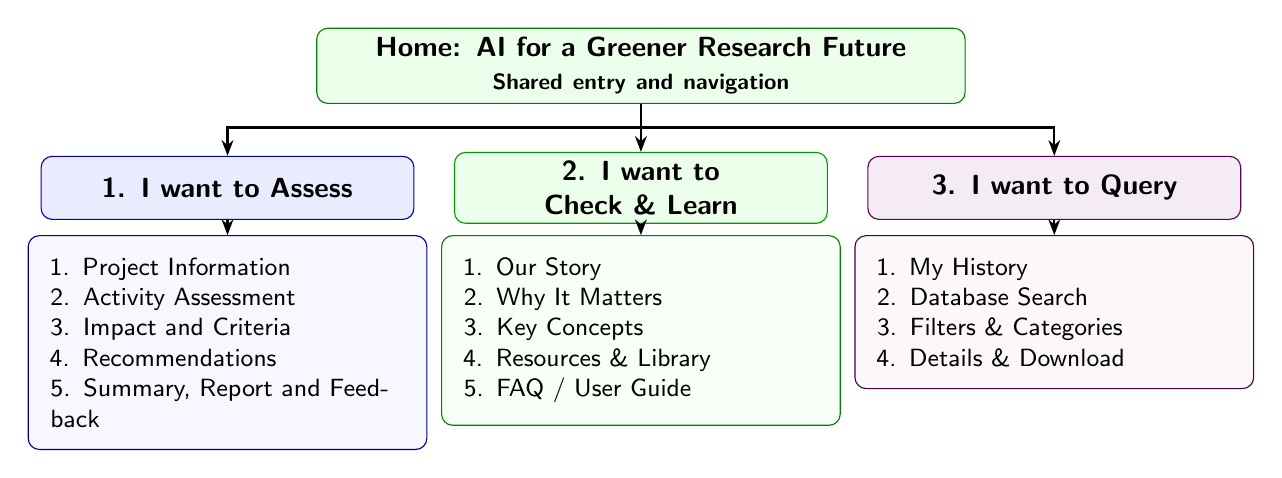
\begin{tikzpicture}[
  every node/.style={font=\sffamily},
  root/.style={draw=green!50!black,fill=green!8,rounded corners,align=center,text width=8cm,minimum height=0.85cm,font=\sffamily\bfseries},
  branch/.style={draw,rounded corners,align=center,text width=4.5cm,minimum height=0.8cm,font=\sffamily\bfseries},
  items/.style={draw,rounded corners,align=left,text width=4.5cm,inner sep=8pt,font=\sffamily\small},
  link/.style={-{Stealth[length=2mm]},thick}]
\node[root] (home) at (0,0) {Home: AI for a Greener Research Future\\\footnotesize Shared entry and navigation};
% ASSESS -- Peng and Yehao may edit this block and its position.
\node[branch,draw=blue!70!black,fill=blue!8] (assess) at (-5.25,-1.55) {1. I want to Assess};
\node[items,draw=blue!55!black,fill=blue!3,anchor=north] (assessitems) at (-5.25,-2.15)
 {1. Project Information\\2. Activity Assessment\\3. Impact and Criteria\\4. Recommendations\\5. Summary, Report and Feedback};
% CHECK & LEARN -- Dennis may edit this block and its position.
\node[branch,draw=green!60!black,fill=green!8] (learn) at (0,-1.55) {2. I want to Check \& Learn};
\node[items,draw=green!50!black,fill=green!3,anchor=north] (learnitems) at (0,-2.15)
 {1. Our Story\\2. Why It Matters\\3. Key Concepts\\4. Resources \& Library\\5. FAQ / User Guide};
% QUERY -- Gerald may edit this block and its position.
\node[branch,draw=violet!70!black,fill=violet!8] (query) at (5.25,-1.55) {3. I want to Query};
\node[items,draw=violet!55!black,fill=violet!3,anchor=north] (queryitems) at (5.25,-2.15)
 {1. My History\\2. Database Search\\3. Filters \& Categories\\4. Details \& Download};
\draw[link] (home.south) -- ++(0,-0.3) -| (assess.north);
\draw[link] (home.south) -- (learn.north);
\draw[link] (home.south) -- ++(0,-0.3) -| (query.north);
\draw[link] (assess.south) -- (assessitems.north);
\draw[link] (learn.south) -- (learnitems.north);
\draw[link] (query.south) -- (queryitems.north);
\end{tikzpicture}}
\caption{Editable information hierarchy and navigation. Detailed processing and ownership appear below; the tree only maps the interface.}
\label{fig:phase2-menu}
\end{figure}

\begin{table}[H]
\centering\small
\begin{tabularx}{\textwidth}{@{}>{\raggedright\arraybackslash}p{0.16\textwidth}>{\raggedright\arraybackslash}p{0.20\textwidth}>{\raggedright\arraybackslash}p{0.34\textwidth}>{\raggedright\arraybackslash}X@{}}
\toprule
Module and purpose & Input & Processing and output & Why it matters \\
\midrule
Home: orient & Goal choice. & Routes to three modules; states advisory scope. & Clear entry and limits. \\
Assess: revise & Project data; Start perception. & AI structures; formulas calculate; criteria support profile, advice and report. & Turns concern into inspectable decisions. \\
Check \& Learn: understand & Question or concept. & Curated explanations, examples and sources. & Explains criteria and gaps. \\
Query: compare & Filters or consented history. & Retrieves reviewed cases with scope and conditions. & Supports valid comparison. \\
\bottomrule
\end{tabularx}
\caption{Module contracts. The exact TU/e web entry point, authentication and maintainer role require client agreement.}
\label{tab:phase2-modules}
\end{table}

\subsection{Current gaps and improvement directions}
TU/e has a sustainability vision and, according to the client Q\&A documented in the retained Phase 1 process appendix, an existing researcher self-assessment. This prototype should complement that practice; its precise integration is unresolved. In a separate US survey of 64 graduate engineering researchers working with AI, 43 reported no environmental impact assessment of their work. Reported reasons included perceived irrelevance or small scale, lack of know-how and competing research priorities. These findings suggest design questions, not measured deficiencies among TU/e researchers \citep{shiekh2026graduate}.
\begin{table}[H]
\centering\footnotesize
\begin{tabularx}{\textwidth}{@{}>{\raggedright\arraybackslash}p{0.16\textwidth}>{\raggedright\arraybackslash}p{0.32\textwidth}>{\raggedright\arraybackslash}p{0.21\textwidth}>{\raggedright\arraybackslash}X@{}}
\toprule
Element & Current status and gap & Evidence & Improvement direction \\
\midrule
Awareness & TU/e has a vision and self-assessment; project-level impacts still need local testing. & Vision; client Q\&A; \citep{shiekh2026graduate}. & Ask for Start perception; show activity quantities; interview TU/e users. \\
Action & Information alone leaves no feasible next step. & \citep{shiekh2026graduate,abrahamse2005review}. & Pair each gap with an action, constraint and source. \\
Explicability & Phase 1 calls for traceability; local factors and boundaries are unspecified. & \citep{friedman2019shaping}. & Expose formula, source version, uncertainty and missing data. \\
Control and privacy & Correction and consent are proposed; reviewer and retention are unassigned. & \citep{santoni2018control,nissenbaum2004privacy}. & Give correction and sharing controls; name a curator. \\
Comparable guidance & Relevant cases may suggest methods; their outcomes depend on activity and boundary. & \citep{oecd2008composite}. & Show case conditions; track change against the researcher's own baseline. \\
\bottomrule
\end{tabularx}
\caption{Gap analysis. The US survey motivates questions for local validation; it is not evidence of TU/e prevalence.}
\label{tab:phase2-gaps}
\end{table}

\subsection{Example user journey and system processing}
% ALL MEMBERS: keep these two lanes aligned with the Phase 1 workflow.
The example user is a researcher planning a six-hour experiment on four GPUs. They want to understand resource use before running it while preserving scientific quality. The journey inherits Phase 1's input, analysis, estimation, comparison, recommendation and feedback sequence.
\begin{figure}[H]
\centering
\resizebox{\textwidth}{!}{%
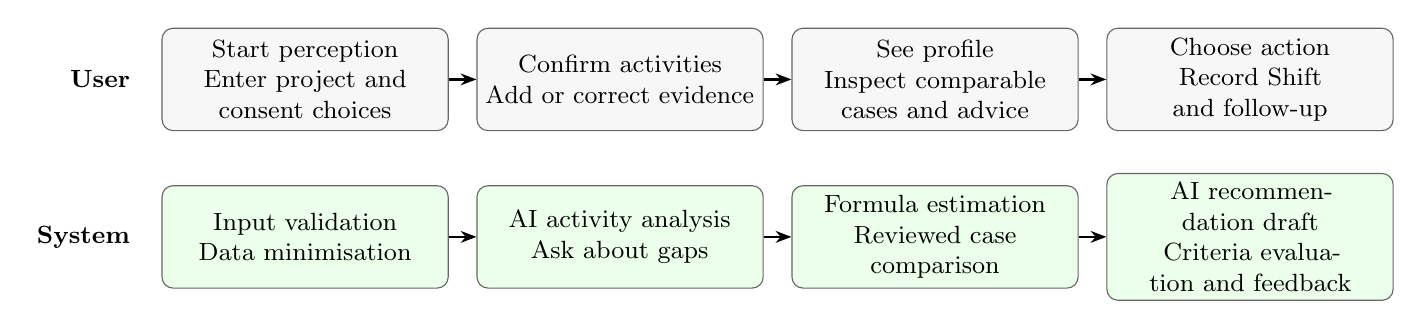
\begin{tikzpicture}[box/.style={draw=black!60,rounded corners,fill=black!3,text width=3.4cm,minimum height=1.3cm,align=center,font=\small},arr/.style={-{Stealth[length=2mm]},thick}]
\node[box] (u1) at (0,0) {Start perception\\Enter project and consent choices};
\node[box] (u2) at (4.0,0) {Confirm activities\\Add or correct evidence};
\node[box] (u3) at (8.0,0) {See profile\\Inspect comparable cases and advice};
\node[box] (u4) at (12.0,0) {Choose action\\Record Shift and follow-up};
\draw[arr] (u1)--(u2);\draw[arr] (u2)--(u3);\draw[arr] (u3)--(u4);
\node[box,fill=green!8] (s1) at (0,-2.0) {Input validation\\Data minimisation};
\node[box,fill=green!8] (s2) at (4.0,-2.0) {AI activity analysis\\Ask about gaps};
\node[box,fill=green!8] (s3) at (8.0,-2.0) {Formula estimation\\Reviewed case comparison};
\node[box,fill=green!8] (s4) at (12.0,-2.0) {AI recommendation draft\\Criteria evaluation and feedback};
\draw[arr] (s1)--(s2);\draw[arr] (s2)--(s3);\draw[arr] (s3)--(s4);
\node[anchor=east,font=\small\bfseries] at (-2.1,0) {User};
\node[anchor=east,font=\small\bfseries] at (-2.1,-2.0) {System};
\end{tikzpicture}}
\caption{Two views of one workflow. User actions are above; internal processing is below. A correction returns to input validation and recalculation. The detailed optional case-sharing route remains in the retained Phase 1 workflow figure.}
\label{fig:phase2-two-lanes}
\end{figure}
The system identifies activity types and missing fields, performs checkable calculations, retrieves cases only when their boundaries are comparable, and drafts recommendations linked to reviewed sources. A researcher can reject a classification or revise an input; the system then recalculates and records what changed. Missing factors produce a qualified result rather than an invented estimate.

\subsection{Criteria, profile and concrete output}
The assessment follows the researcher's own activity rather than assigning a universal score. It records the scientific purpose, relevant resource use, data quality, a feasible change, and what happened after that change. Quantities retain their units and boundaries; missing information remains unknown. For example, four GPUs used for six hours amount to 24 GPU-hours, but this alone does not establish electricity use or emissions \citep{lacoste2019carbon}.

Table~\ref{tab:phase2-profile} turns five provisional criteria into prompts for a project-specific profile. A comparison is meaningful only when the research outcome, quality requirement, units and system boundary are comparable. A personal target is recorded as the researcher's intention; an observed improvement requires follow-up evidence.
\begin{table}[H]
\centering\small
\begin{tabularx}{\textwidth}{@{}>{\raggedright\arraybackslash}p{0.21\textwidth}>{\raggedright\arraybackslash}p{0.36\textwidth}>{\raggedright\arraybackslash}X@{}}
\toprule
Criterion & Project-specific input and evidence & Personal comparison and output \\
\midrule
C1 Activity boundary and inputs & State the scientific outcome, functional unit, included steps, equipment or materials, amounts, duration, repeats and data sources. & Show relevant quantities with units and exclusions; ask for missing inputs. \\
C2 Comparable alternative & Describe the current method and a feasible alternative that meets the same research-quality requirement. & Compare with this project's baseline only where boundaries and evidence match; otherwise explain why comparison is pending. \\
C3 Avoidable use & Record failed or repeated runs, idle equipment or material loss, and a feasible action or pilot. & Identify a specific opportunity and action; record the result after testing. \\
C4 Wider impacts and total use & Include total runs or samples, other relevant energy, materials and waste, and any change in project scope. & Check whether a local saving shifts impacts or reduces total project use. \\
C5 Follow-up and revision & Keep the baseline, personal target, review date, comparable follow-up data and explanation of changes. & Show baseline, action and observed outcome separately; revise advice when evidence changes. \\
\bottomrule
\end{tabularx}
\caption{Provisional activity-specific assessment prompts, adapted from the team's tutor-meeting outline. Measured values, sourced estimates and unknowns remain distinct. The criteria do not imply thresholds, weights, a ranking or an overall score.}
\label{tab:phase2-profile}
\end{table}
\begin{center}
\fcolorbox{blue!65!black}{blue!3}{\begin{minipage}{0.91\textwidth}
\textbf{Illustrative GPU-computation profile}\\
\textbf{Purpose and boundary:} One successful run at the required scientific quality; also track all project runs.\\
\textbf{Current record:} Four GPUs for six hours (24 GPU-hours); electricity and emissions unknown without suitable power and facility data.\\
\textbf{Personal aim:} Test whether a smaller configuration can deliver the same result with less total electricity.\\
\textbf{What is missing?} Measured or defensible power, utilisation, failed runs and total planned runs.\\
\textbf{Next action:} Pilot a comparable configuration and record energy, run count and research quality.\\
\textbf{Observed improvement:} Pending follow-up; a projected saving is not presented as a measured result.\\
\textbf{Controls:} [Correct] [Challenge] [Save privately] [Review ``Case A'' for sharing].
\end{minipage}}
\end{center}

The output keeps environmental quantities, evidence quality and goal progress separate. The five criteria are prompts for tailored feedback, not a scale to add or average. A laboratory battery batch could instead track material losses and valid samples; a printed prototype could track failed prints and acceptable parts. In each case, advice must preserve scientific quality and safety. Cross-project examples may inform methods, but do not provide a ranking. Weighting unlike indicators into one number would require value judgements the group has not established \citep{oecd2008composite}.

\subsection{Start--Shift: project-specific progress}
The researcher records an initial activity and a personal goal. The system identifies relevant quantities and evidence gaps, then suggests a feasible action. At a later visit, the researcher can enter comparable measurements and explain changes in research scope or quality. Figure~\ref{fig:start-shift-loop} separates the first usable advice from optional follow-up; expected and observed outcomes remain distinct.
\begin{figure}[!htbp]
\centering
\begin{minipage}[t]{0.43\textwidth}
\centering
\textbf{Core path and optional return}\\[-0.1em]
\resizebox{\linewidth}{!}{%
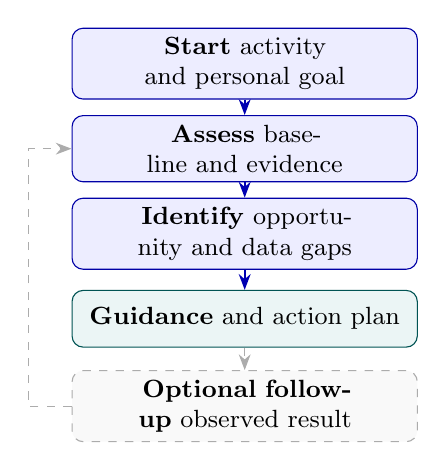
\begin{tikzpicture}[
  core/.style={draw=blue!65!black,fill=blue!7,rounded corners,align=center,text width=4.15cm,minimum height=0.72cm,font=\small},
  choice/.style={draw=teal!65!black,fill=teal!8,rounded corners,align=center,text width=4.15cm,minimum height=0.72cm,font=\small},
  future/.style={draw=gray!65,dashed,fill=gray!5,rounded corners,align=center,text width=4.15cm,minimum height=0.68cm,font=\small},
  flow/.style={-{Stealth[length=2mm]},thick,draw=blue!70!black},
  revisit/.style={-{Stealth[length=2mm]},dashed,draw=gray!65}]
\node[core] (start) at (0,0) {\textbf{Start} activity and personal goal};
\node[core] (assess) at (0,-1.08) {\textbf{Assess} baseline and evidence};
\node[core] (gap) at (0,-2.16) {\textbf{Identify} opportunity and data gaps};
\node[choice] (advice) at (0,-3.24) {\textbf{Guidance} and action plan};
\node[future] (follow) at (0,-4.35) {\textbf{Optional follow-up} observed result};
\draw[flow] (start)--(assess);
\draw[flow] (assess)--(gap);
\draw[flow] (gap)--(advice);
\draw[revisit] (advice)--(follow);
\draw[revisit] (follow.west) -- ++(-0.55,0) |- (assess.west);
\end{tikzpicture}}
\end{minipage}\hfill
\begin{minipage}[t]{0.53\textwidth}
\centering
\textbf{Versioned phase matrix}\\[-0.1em]
\footnotesize
\begin{tabularx}{\linewidth}{@{}>{\raggedright\arraybackslash}p{0.28\linewidth}>{\raggedright\arraybackslash}X@{}}
\toprule
Stage & Illustrative GPU-computation record \\
\midrule
Baseline & Four GPUs for six hours; 24 GPU-hours \\
Evidence gap & Electricity, failed runs and total runs unknown \\
Goal & Same research quality with less total electricity \\
Action & Pilot fewer GPUs; measure comparable runs \\
Expected & Possible saving; no measured gain yet \\
Follow-up & Record actual energy, quality and total use \\
\bottomrule
\end{tabularx}
\end{minipage}
\caption{Solid blue arrows show the first usable result; muted dashed arrows mean a second or third assessment may occur, but is not required. Each relevant criterion can keep separate stage records, assumptions and source versions if the user chooses private storage. An estimate, a target and an observed improvement are different kinds of information; unknowns remain unknown.}
\label{fig:start-shift-loop}
\end{figure}
Goal-reference research supports presenting change relative to a meaningful target: people evaluate gains and shortfalls relative to reference points, rather than only final totals \citep{kahneman1979prospect,heath1999goals}. Formative-feedback work supports specific next steps rather than a terminal grade; self-regulation and personal-informatics models describe iterative, stage-based reflection and action \citep{shute2008feedback,zimmerman2002self,li2010stages}. These are design analogies, not evidence that this display will improve TU/e research behaviour. Comprehension, discouragement and actual follow-up must be tested \citep{carver1982control,hattie2007feedback}.

Consented cases from a proposed restricted repository could offer examples of feasible methods when activity and research-quality requirements match. This addresses the gap between general sustainability knowledge and locally relevant action illustrated by the graduate survey \citep{shiekh2026graduate}. Such examples would give context for the researcher's own decision, without ranking projects or researchers. TU/e could separately consider recognition for verified improvements, but awards or institutional incentives require their own governance.

\subsection{Explicability, human control and privacy}
The proposed knowledge base has three reviewed layers: authoritative TU/e guidance where applicable, published factors with scope and date, and consented cases whose conditions and outcomes have been checked. AI may classify activities, retrieve and summarise sources, propose comparators and draft suggestions. It may not create official policy, approve an archive entry or alter criteria without review. Fixed formulas perform arithmetic; an authorised maintainer validates source updates and can withdraw outdated advice. This separation makes outcomes traceable to both evidence and responsible people, reflecting the course's explicability and meaningful-human-control themes \citep{friedman2019shaping,santoni2018control,eu_ethics_2021}.

The researcher chooses the detail entered, may omit unpublished or industry-confidential information, confirms AI-extracted activities, corrects assumptions, accepts or rejects advice, and chooses separately whether to save a private result, contribute to aggregate comparison, or share a reviewed case. Self-assessment remains available without archive sharing. The owner can recognise their own record; other users see only a consented, redacted case under a code (e.g., ``Case A'') or a sufficiently broad aggregate. A designated data steward would keep any identity--code mapping separately with restricted access; curators need only the case code and approved summary. Small groups and distinctive project details should be suppressed when they permit inference. A code is \emph{pseudonymisation}, not guaranteed anonymity: linkable records remain personal data \citep{edpb2025pseudonymisation,gdpr2016}. This design applies purpose limitation, data minimisation and privacy by default, while leaving retention periods, legal basis and access roles for TU/e to determine \citep{gdpr2016,nissenbaum2004privacy}. A source challenge goes to a named reviewer and is not silently learned from as truth.

\subsection{Evidence-to-design rationale}
The source-to-design links are concentrated in Table~\ref{tab:phase2-gaps}. The US graduate survey motivates activity prompts and actionable guidance, but requires local testing \citep{shiekh2026graduate}. VSD makes explicability, autonomy and environmental impact design values to investigate with stakeholders rather than merely interface labels \citep{friedman2019shaping}. Feedback theory motivates Start--Shift, while meaningful human control and contextual privacy justify correction, curator review and separate sharing choices \citep{carver1982control,hattie2007feedback,santoni2018control,nissenbaum2004privacy}. OECD/JRC guidance supports keeping criteria visible and avoiding unsupported aggregation \citep{oecd2008composite}.

\subsection{Interface}
\label{sec:phase2-interface}
The interface will be designed as a simple web-based tool with three main functions: I want to Assess, I want to Check \& Learn, and I want to Query. The homepage will provide a clear overview of these functions so that researchers can choose between assessing their own research, learning more about sustainability, or exploring previous records and available resources.

The Assess function is the main AI-based part of the tool. The researcher first provides information about their research project, such as the type of research, activities, equipment, duration and other relevant details. The AI analyses this information and asks follow-up questions when important information is missing. It then identifies possible sustainability impacts and provides explanations and recommendations. The results can include aspects such as energy use, carbon emissions and other environmental impacts. The researcher can review the results, correct information or assumptions made by the AI, and then receive a final summary and guidance. The assessment is intended to support self-reflection and is not an official sustainability certification or approval.

The Check \& Learn function provides the knowledge behind the assessment. It contains an introduction to the purpose of the tool, explanations of the connection between research and sustainability, key sustainability concepts, and a Sustainability Library. The library will contain guidelines, scientific literature, case studies, sustainability frameworks, relevant databases and external resources. Sources should come from reliable and reviewed sources, such as TU/e sustainability policies and guidelines, scientific publications, recognised sustainability organisations and relevant environmental databases. Each source can include information about its origin, publication or update date, scope and relevance to the assessment. This makes it possible for researchers to understand where the information comes from and to investigate the topic further.

The library will also contain examples of research activities and their possible sustainability impacts. These examples can help researchers understand how sustainability considerations can apply to different types of research. The AI can use the information from the reviewed knowledge base when analysing a research project and refer the researcher to the relevant sources. This means that the AI does not have to generate all sustainability information itself, but can use the library as a controlled source of knowledge. New sources can be added and existing sources can be reviewed or updated by designated sustainability experts. The AI itself should not independently add information to the official knowledge base.

The Query function allows researchers to explore information beyond their current assessment. Researchers can view their own previous assessments and search the available database using filters such as research field, impact type or keywords. They can also explore relevant case studies, datasets, best practices and policies. When appropriate, comparable previous cases can help researchers understand how similar research activities have considered sustainability. Detailed information and relevant resources can be viewed or downloaded. Any sharing of research records should be subject to appropriate consent and privacy controls.

The interface will use clear headings, buttons and information cards. The three main functions will be visually separated so users can understand each purpose. Researcher input, AI-generated suggestions and retrieved records will be visually distinguished. The three walkthroughs are proposed screens for team review; Dennis will refine the Check \& Learn content and its source presentation.


\subsection{Evaluation plan and team responsibilities}
The prototype will be compared with a structured non-AI checklist on the same test cases, as proposed in Phase 1. Measures are absolute calculation error, the share of recommendations supported by reviewed sources, the share of users who can explain a criterion, task completion and correction time, correct handling of sharing choices, and the share of suggestions judged feasible by domain reviewers. A separate test should compare a static profile with the profile-plus-gap display on comprehension, chosen action and later follow-up. Thresholds and reviewers must be agreed before testing; no result is claimed here.
\begin{table}[H]
\centering\small
\begin{tabularx}{\textwidth}{@{}>{\raggedright\arraybackslash}p{0.21\textwidth}>{\raggedright\arraybackslash}p{0.39\textwidth}X@{}}
\toprule
Member & Lead responsibility & Shared work or handoff \\
\midrule
Yehao Chen & Overall workflow, core concepts and shared navigation. & Assess steps and follow-up loop with Peng. \\
Dennis de Hoon & Check \& Learn: Our Story, Why It Matters, Library and FAQ. & Explanations and source cards linked to Assess. \\
Peng Wang & Assessment criteria, interface and data presentation. & Assess steps and follow-up loop with Yehao. \\
Gerald Tobenna Eluagu & Query and history: records, search, filters and sharing controls. & Connect past records and reviewed cases to Assess. \\
\bottomrule
\end{tabularx}
\caption{Current Phase 2 responsibilities and the shared Assess workflow.}
\label{tab:phase2-owners}
\end{table}

% END embedded Mock-up.tex

\clearpage
\begin{thebibliography}{18}
\providecommand{\natexlab}[1]{#1}
\providecommand{\url}[1]{\texttt{#1}}
\expandafter\ifx\csname urlstyle\endcsname\relax
  \providecommand{\doi}[1]{doi: #1}\else
  \providecommand{\doi}{doi: \begingroup \urlstyle{rm}\Url}\fi

\bibitem[Abrahamse et~al.(2005)Abrahamse, Steg, Vlek, and
  Rothengatter]{abrahamse2005review}
Wokje Abrahamse, Linda Steg, Charles Vlek, and Talib Rothengatter.
\newblock A review of intervention studies aimed at household energy
  conservation.
\newblock \emph{Journal of Environmental Psychology}, 25\penalty0 (3):\penalty0
  273--291, 2005.
\newblock \doi{10.1016/j.jenvp.2005.08.002}.

\bibitem[Carver and Scheier(1982)]{carver1982control}
Charles~S. Carver and Michael~F. Scheier.
\newblock Control theory: A useful conceptual framework for personality-social,
  clinical, and health psychology.
\newblock \emph{Psychological Bulletin}, 92\penalty0 (1):\penalty0 111--135,
  1982.
\newblock \doi{10.1037/0033-2909.92.1.111}.

\bibitem[{Eindhoven University of Technology}(2023)]{tue_sustainability_2021}
{Eindhoven University of Technology}.
\newblock Tu/e sustainability visioning report.
\newblock Technical report, TU/e Sustainability Ambassador Office, 2023.
\newblock URL
  \url{https://assets.w3.tue.nl/w/fileadmin/TU_e_Sustainability/Sustainability_Team/Logos/TUe%20Sustainability%20Visioning%20Report%20Spread.pdf}.

\bibitem[{European Commission}(2021)]{eu_ethics_2021}
{European Commission}.
\newblock Ethics by design and ethics of use approaches for artificial
  intelligence.
\newblock Technical report, Directorate-General for Research and Innovation,
  2021.
\newblock URL
  \url{https://ec.europa.eu/info/funding-tenders/opportunities/docs/2021-2027/horizon/guidance/ethics-by-design-and-ethics-of-use-approaches-for-artificial-intelligence_he_en.pdf}.

\bibitem[{European Data Protection Board}(2025)]{edpb2025pseudonymisation}
{European Data Protection Board}.
\newblock Guidelines 01/2025 on pseudonymisation (version for public
  consultation), 2025.
\newblock URL
  \url{https://www.edpb.europa.eu/system/files/2025-01/edpb_guidelines_202501_pseudonymisation_en.pdf}.

\bibitem[{European Parliament and Council of the European
  Union}(2016)]{gdpr2016}
{European Parliament and Council of the European Union}.
\newblock Regulation (eu) 2016/679 (general data protection regulation), 2016.
\newblock URL \url{https://eur-lex.europa.eu/eli/reg/2016/679/oj/eng}.

\bibitem[Friedman and Hendry(2019)]{friedman2019shaping}
Batya Friedman and David~G. Hendry.
\newblock \emph{Value Sensitive Design: Shaping Technology with Moral
  Imagination}.
\newblock MIT Press, 2019.

\bibitem[Hattie and Timperley(2007)]{hattie2007feedback}
John Hattie and Helen Timperley.
\newblock The power of feedback.
\newblock \emph{Review of Educational Research}, 77\penalty0 (1):\penalty0
  81--112, 2007.
\newblock \doi{10.3102/003465430298487}.

\bibitem[Heath et~al.(1999)Heath, Larrick, and Wu]{heath1999goals}
Chip Heath, Richard~P. Larrick, and George Wu.
\newblock Goals as reference points.
\newblock \emph{Cognitive Psychology}, 38\penalty0 (1):\penalty0 79--109, 1999.
\newblock \doi{10.1006/cogp.1998.0708}.

\bibitem[Kahneman and Tversky(1979)]{kahneman1979prospect}
Daniel Kahneman and Amos Tversky.
\newblock Prospect theory: An analysis of decision under risk.
\newblock \emph{Econometrica}, 47\penalty0 (2):\penalty0 263--291, 1979.
\newblock \doi{10.2307/1914185}.

\bibitem[Lacoste et~al.(2019)Lacoste, Luccioni, Schmidt, and
  Dandres]{lacoste2019carbon}
Alexandre Lacoste, Alexandra Luccioni, Victor Schmidt, and Thomas Dandres.
\newblock Quantifying the carbon emissions of machine learning.
\newblock arXiv preprint arXiv:1910.09700, 2019.

\bibitem[Li et~al.(2010)Li, Dey, and Forlizzi]{li2010stages}
Ian Li, Anind Dey, and Jodi Forlizzi.
\newblock A stage-based model of personal informatics systems.
\newblock In \emph{Proceedings of the SIGCHI Conference on Human Factors in
  Computing Systems}, pages 557--566. ACM, 2010.
\newblock \doi{10.1145/1753326.1753409}.

\bibitem[Nissenbaum(2004)]{nissenbaum2004privacy}
Helen Nissenbaum.
\newblock Privacy as contextual integrity.
\newblock \emph{Washington Law Review}, 79\penalty0 (1):\penalty0 119--157,
  2004.
\newblock URL \url{https://digitalcommons.law.uw.edu/wlr/vol79/iss1/10/}.

\bibitem[{OECD} and {European Commission Joint Research
  Centre}(2008)]{oecd2008composite}
{OECD} and {European Commission Joint Research Centre}.
\newblock \emph{Handbook on Constructing Composite Indicators: Methodology and
  User Guide}.
\newblock OECD Publishing, Paris, 2008.
\newblock \doi{10.1787/9789264043466-en}.

\bibitem[Santoni~de Sio and van~den Hoven(2018)]{santoni2018control}
Filippo Santoni~de Sio and Jeroen van~den Hoven.
\newblock Meaningful human control over autonomous systems: A philosophical
  account.
\newblock \emph{Frontiers in Robotics and AI}, 5:\penalty0 15, 2018.
\newblock \doi{10.3389/frobt.2018.00015}.

\bibitem[Shiekh and Zhu(2026)]{shiekh2026graduate}
Kylee Shiekh and Qin Zhu.
\newblock Exploring how graduate engineering researchers approach {AI}
  sustainability: Perceptions, design considerations, and impact assessment.
\newblock \emph{International Journal of Technology and Design Education},
  2026.
\newblock \doi{10.1007/s10798-026-10100-y}.
\newblock URL
  \url{https://link.springer.com/article/10.1007/s10798-026-10100-y}.

\bibitem[Shute(2008)]{shute2008feedback}
Valerie~J. Shute.
\newblock Focus on formative feedback.
\newblock \emph{Review of Educational Research}, 78\penalty0 (1):\penalty0
  153--189, 2008.
\newblock \doi{10.3102/0034654307313795}.

\bibitem[Zimmerman(2002)]{zimmerman2002self}
Barry~J. Zimmerman.
\newblock Becoming a self-regulated learner: An overview.
\newblock \emph{Theory Into Practice}, 41\penalty0 (2):\penalty0 64--70, 2002.
\newblock \doi{10.1207/s15430421tip4102_2}.

\end{thebibliography}

\end{document}
